\section{Metode}
\subsection{Utstyr}
\begin{itemize}
    \item Telefoner med Phyphox
    \item Telefonholder
    \item Trefot
    \item Vater
\end{itemize}
Det ble foretatt målinger med Djupviks iPhone SE, Jakobsens Samsung Galaxy A40 og Aakres iPhone 13. 

\subsection{Referansepunkter og målelokasjon}
Det ble gjort målinger med 2 ulike referansepunkt for å bedre datagrunnlag. De valgte referansepunktene var Nidarosdomen og Tyholttårnet, se figur 2\ref{fig:angle_north}. Koordinatene til referansepunktene ble bestemt via Google Maps. Koordinatene til målelokasjonen ble målt ved hjelp av Phyphox \cite{phyphox}. Telefonene ble kalibrert ved at de ble beveget noen meter i hver retning. Deretter ble de plassert i ro ved målelokasjon til målingen stabiliserte seg. Målingene ble utført på vestre siden av broen som krysser Eidsvolls gate langs Øvre alle. 


\subsection{Måling av magnetfelt og oppsett}
En trefot med en plattform for telefonene ble brukt, hvor telefonene ble plassert i en telefonholder. For å gi riktig retning på telefonene, ble det plassert ett vater langsmed telefonholderen \ref{fig:med_vater}. Vateret ble så brukt som siktemiddel slik at telefonholderen, og dermed telefonen lå i retning av referansepunktet. Deretter ble plattformen justert slik at den var horisontal ved hjelp av et vater.

Før hver måling ble telefonene kalibrert ved å rotere de rundt alle tre aksene. Deretter ble telefonene plassert i telefonholderen og ble liggende der til målingene (rundt $30$ sekunder). Dataene ble så eksportert til \kode{.csv}-format. 

Måling med Nidarosdomen som referansepunkt ble gjennomført først. Det ble gjennomført et målesett (en måling med hver telefon). Deretter ble plattformen stilt inn på nytt med Tyholttårnet som referansepunkt. Det ble gjort målinger med flymodus aktivert og etter å ha gjort en omstart av telefonene for å sjekke om dette kunne ha innvirkning på resultatene. Målingene med flymodus ble gjennomført ved at telefonene ble satt i flymodus, kalibrert og dermed satt i telefonholderen. Målingene etter omstart ble gjennomført ved at telefonene ble startet på nytt, kalibrert og så plassert i telefonholderen.

For å finne koordinatene til målelokasjonen ble Phyphox' verktøy for GPS-sensoren til mobilen benyttet. GPS-sensoren ble kalibrert ved at de ble flyttet noen meter i ulike retninger før selve målingen ble utført i telefonholderen. Lokasjonsdataene ble eksportert i \kode{.csv}-format.

\subsubsection{Analyse av data}
Rådata for magnetfeltet og koordinatene til målelokasjonen ble gruppert for målesett og person.
Inklinasjonen ble bestemt ved bruke \eqref{eq:inclination} på hvert datasett, samt bruke funksjonene \kode{numpy.mean}, \kode{numpy.median} og \kode{sympy.stats.tstd} for å finne gjennomsnittet, medianen og standardavviket.
Deretter ble vinkelen mellom referansepunkt og geografisk nord ($\theta$) regnet ut for hver person ved å bruke \kode{geodesic.Geodesic.WGS84.Inverse()} fra geographiclib-biblioteket.
Innsatt i \eqref{eq:declination} gir dette sluttresultatet for hvert målesett.
Til slutt ble alle dataene samlet i et målesett og analysert i sin helhet med metoden som beskrevet over. Måledataene til Vemund for Nidarosdomen ble deretter filtret ut og en ny analyse ble gjennomført.   

 
\begin{figure}
    \centering
    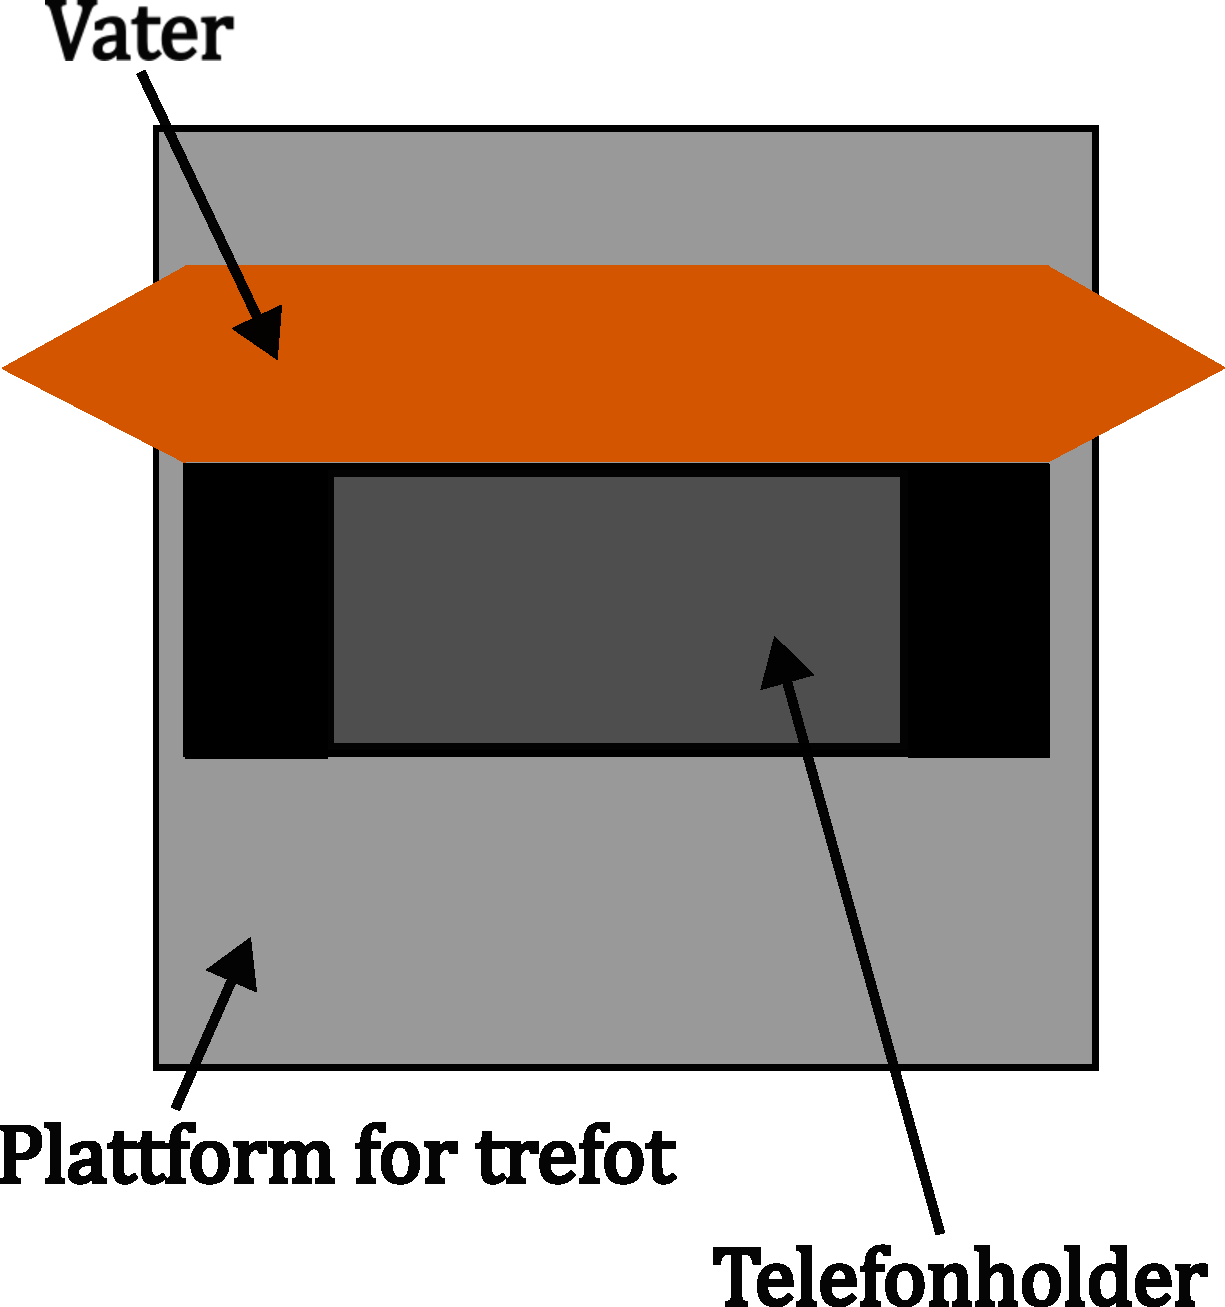
\includegraphics[width=0.45\textwidth]{img/Plattform med vater.pdf}                 
    \caption{Figuren viser oppsettet for måling før telefonen ble plassert i telefonholderen. Vateret er siktemiddel for referansepunktet.}
    \label{fig:med_vater}
\end{figure}

\begin{figure}
    \centering
    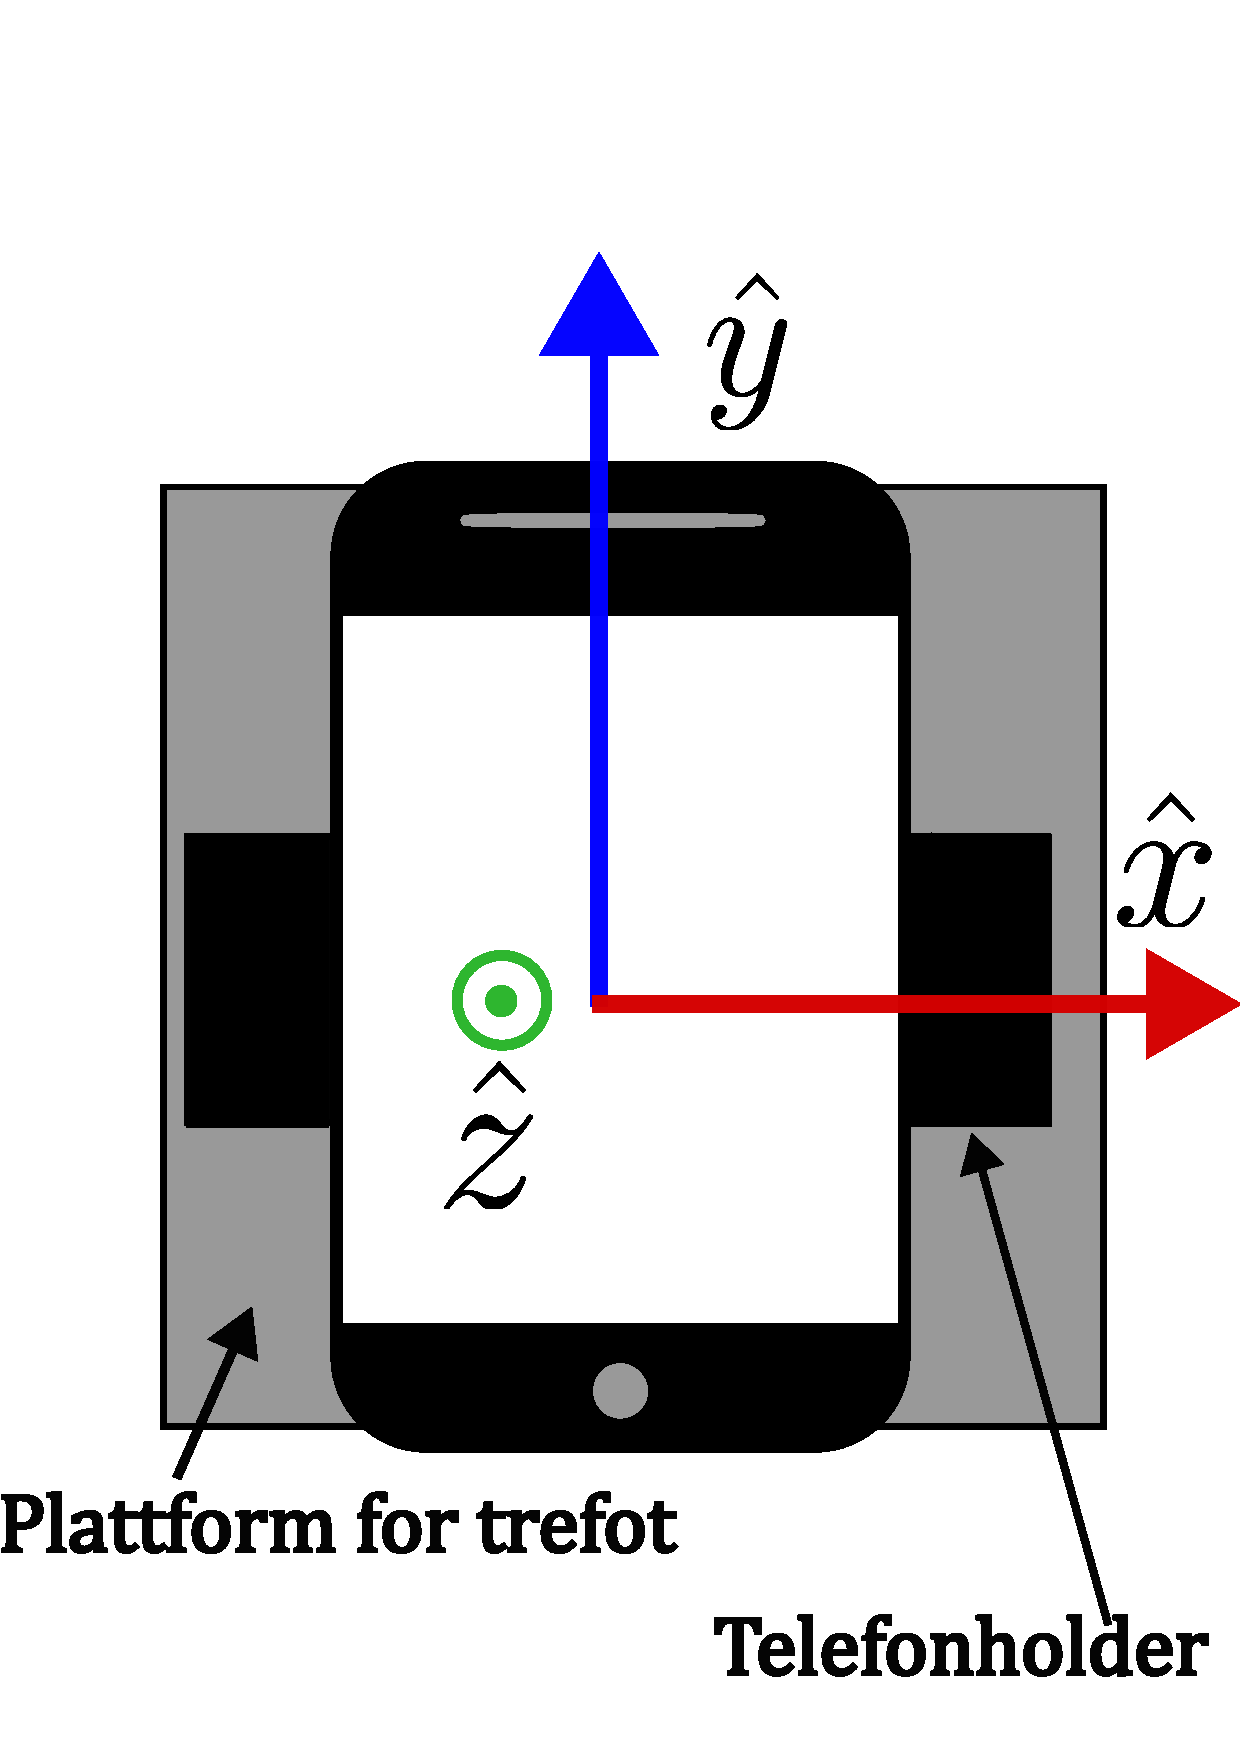
\includegraphics[width=0.65\textwidth]{img/Plattform med telefoni.pdf}
    \caption{Referansesystem for målinger foretatt med telefon satt i telefonholder.}
    \label{fig:telf_akser}
\end{figure}